\documentclass[12pt]{article}

\usepackage[margin=1in]{geometry} 
\usepackage{amsmath,amsthm,amssymb}
\usepackage[spanish]{babel}
\usepackage[utf8]{inputenc}
\usepackage{tikz-cd}
\usepackage{amsmath}
\usepackage[shortlabels]{enumitem}
\usepackage{mathtools}
\usepackage{float}
\usepackage{listings}
\usepackage{xcolor}


\graphicspath{{img/}}

\title{SWAP: Práctica 3}
\author{
        Antonio Gámiz Delgado
}

\begin{document}
\maketitle

\section{Configuración del entorno}

\subsection{Configuración de M3}

Como las máquinas \textit{M1} y \textit{M2} ya se encuentran configuaradas, primero crearemos y configuraremos la máquina que hará de balanceador de carga, \textit{M3}:

\begin{figure}[H]
\center
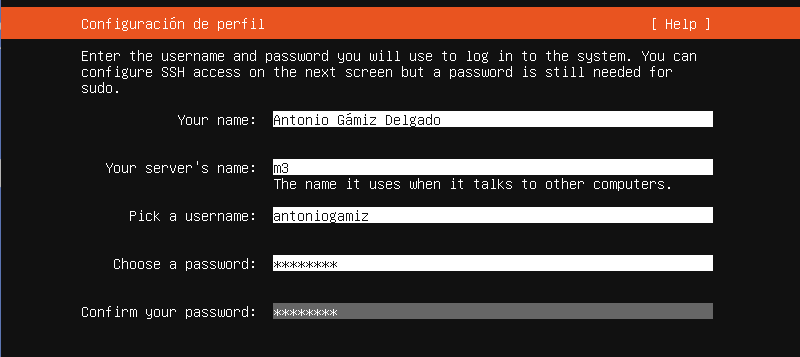
\includegraphics[scale=0.5]{1.png}
\end{figure}

Tenemos que repetir los pasos de la práctica 1 para conectar la máquina \textit{M3} a la red:

\begin{figure}[H]
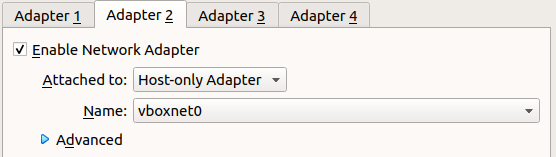
\includegraphics[scale=0.5]{2.png}
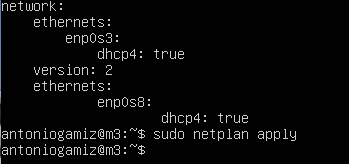
\includegraphics[scale=0.5]{3.png}
\end{figure}

Ya tenemos la máquina lista para usar con \textit{ssh}. Para aclarar, las IPs de cada máquina son:
\begin{itemize}
\item M1=192.168.56.102
\item M2=192.168.56.103
\item M3=192.168.56.104
\end{itemize}

\subsection{Balanceador: nginx}

Ahora instalamos \textit{nginx} en \textit{M3}:\medskip

\begin{figure}[H]
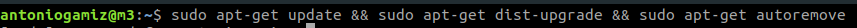
\includegraphics[scale=0.5]{4.png}
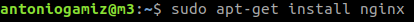
\includegraphics[scale=0.5]{5.png}
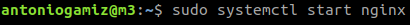
\includegraphics[scale=0.5]{6.png}
\end{figure}

Una vez instalado procedemos a la configuración. Escribimos el siguiente texto en el archivo \textit{/etc/nginx/conf.d/default.conf}

\begin{figure}[H]
\center
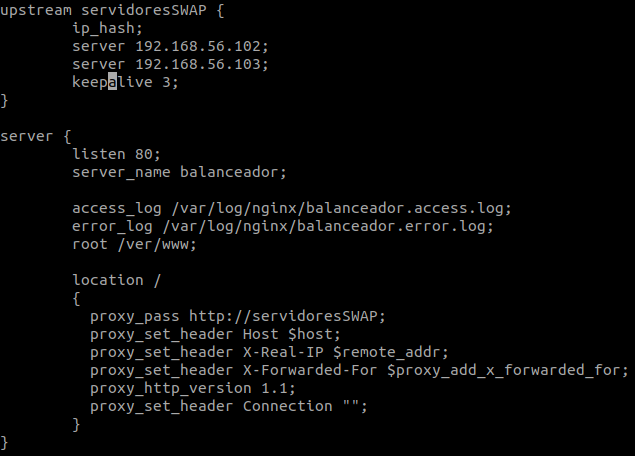
\includegraphics[scale=0.5]{7.png}
\end{figure}

Debido a que \textit{nginx} no está funcionando como balanceador he tenido que aplicar la solución propuesta en el guión:

\begin{figure}[H]
\center
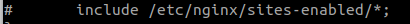
\includegraphics[scale=0.5]{9.png}
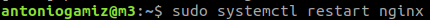
\includegraphics[scale=0.5]{10.png}
\end{figure}

Y ya todo funciona correctamente:

\begin{figure}[H]
\center
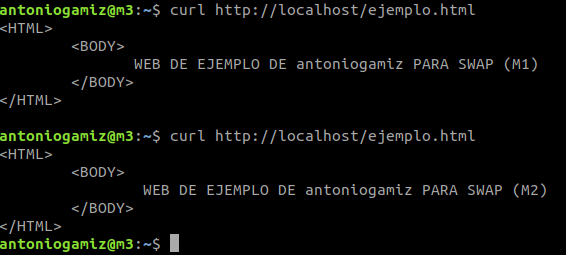
\includegraphics[scale=0.5]{11.png}
\end{figure}

Ahora probamos la opción de \textit{weight} y vemos que funciona correctamente:

\begin{figure}[H]
\center
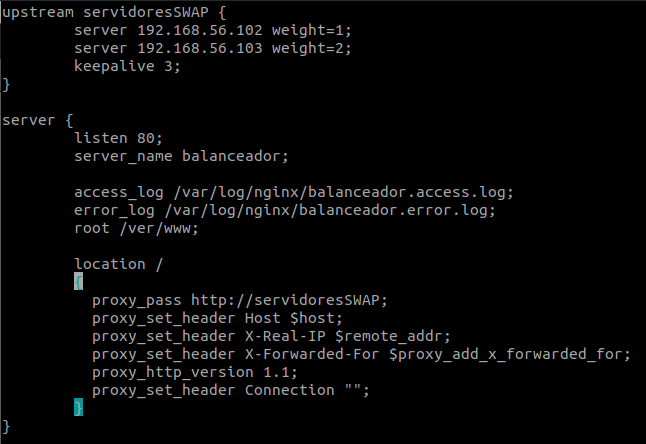
\includegraphics[scale=0.5]{22.png}
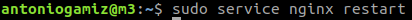
\includegraphics[scale=0.6]{23.png}
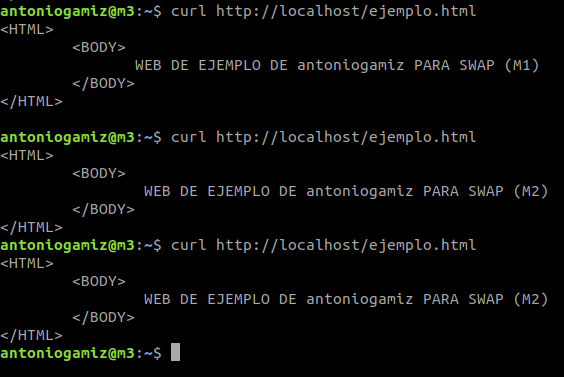
\includegraphics[scale=0.5]{24.png}
\end{figure}




\subsection{Balanceador: haproxy}

\begin{figure}[H]
\center
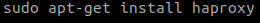
\includegraphics[scale=0.5]{12.png}
\end{figure}

Configuramos \textit{haproxy} modificando el archivo \textit{/etc/haproxy/haproxy.cfg}:

\begin{figure}[H]
\center
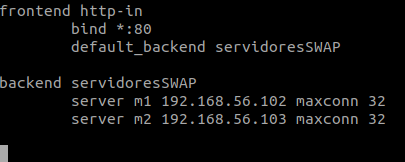
\includegraphics[scale=0.5]{13.png}
\end{figure}

Apagamos \textit{nginx} y arrancamos \textit{haproxy}:

\begin{figure}[H]
\center
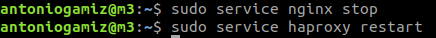
\includegraphics[scale=0.5]{14.png}
\end{figure}

Comprobamos que todo funciona correctamente:

\begin{figure}[H]
\center
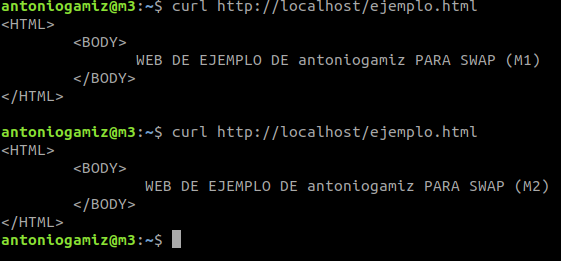
\includegraphics[scale=0.5]{15.png}
\end{figure}

\subsection{Balanceador: lighty }

Instalamos \textit{lighttpd}:

\begin{figure}[H]
\center
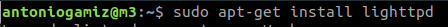
\includegraphics[scale=0.5]{25.png}
\end{figure}

El archivo de configuración se encuentra en \textit{/etc/lighttpd/lighttpd.conf}. Tenemos que añadir \textit{mod\_proxy} a la lista de \textit{server.modules}:

\begin{figure}[H]
\center
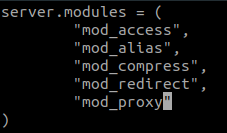
\includegraphics[scale=0.5]{26.png}
\end{figure}

Ahora tenemos que añadir un archivo a \textit{/etc/lighttpd/conf-enabled} con la configuración necesaria para el balanceo de carga:

\begin{figure}[H]
\center
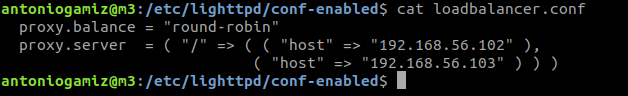
\includegraphics[scale=0.5]{27.png}
\end{figure}

Nos aseguramos de que los otros dos balanceadores de carga están apagados y arrancamos \textit{lighttpd}:

\begin{figure}[H]
\center
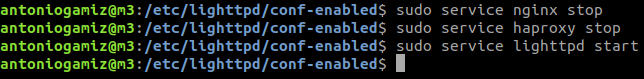
\includegraphics[scale=0.5]{28.png}
\end{figure}

Hacemos un par de peticiones con \textit{curl} para ver que funciona correctamente:

\begin{figure}[H]
\center
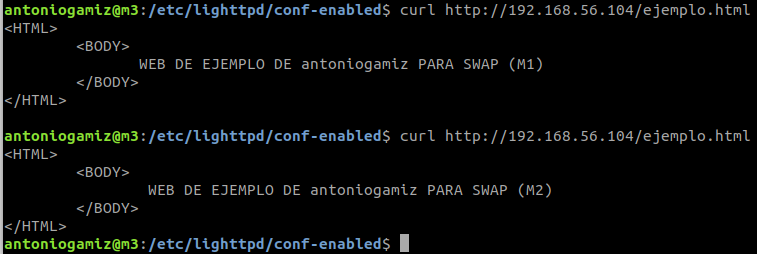
\includegraphics[scale=0.5]{29.png}
\end{figure}


\section{Benchmarking}

Una vez que tenemos todo configurado, es hora de empezar a hacer pruebas. Empezamos por instalar la utilidad \textit{ab} en \textit{M3} (viene con \textit{Apache}, pero en \textit{M3} no está instalado \textit{Apache}):

\begin{figure}[H]
\center
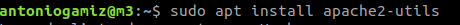
\includegraphics[scale=0.5]{16.png}
\end{figure}

Recordemos que el \textit{benchmark} tiene que ser ejecutado en otra máquina diferente a \textit{M3} (yo he usado el host de la máquina virtual).

\subsection{Haproxy}

Ejecución de \textit{ab}:

\begin{figure}[H]
\center
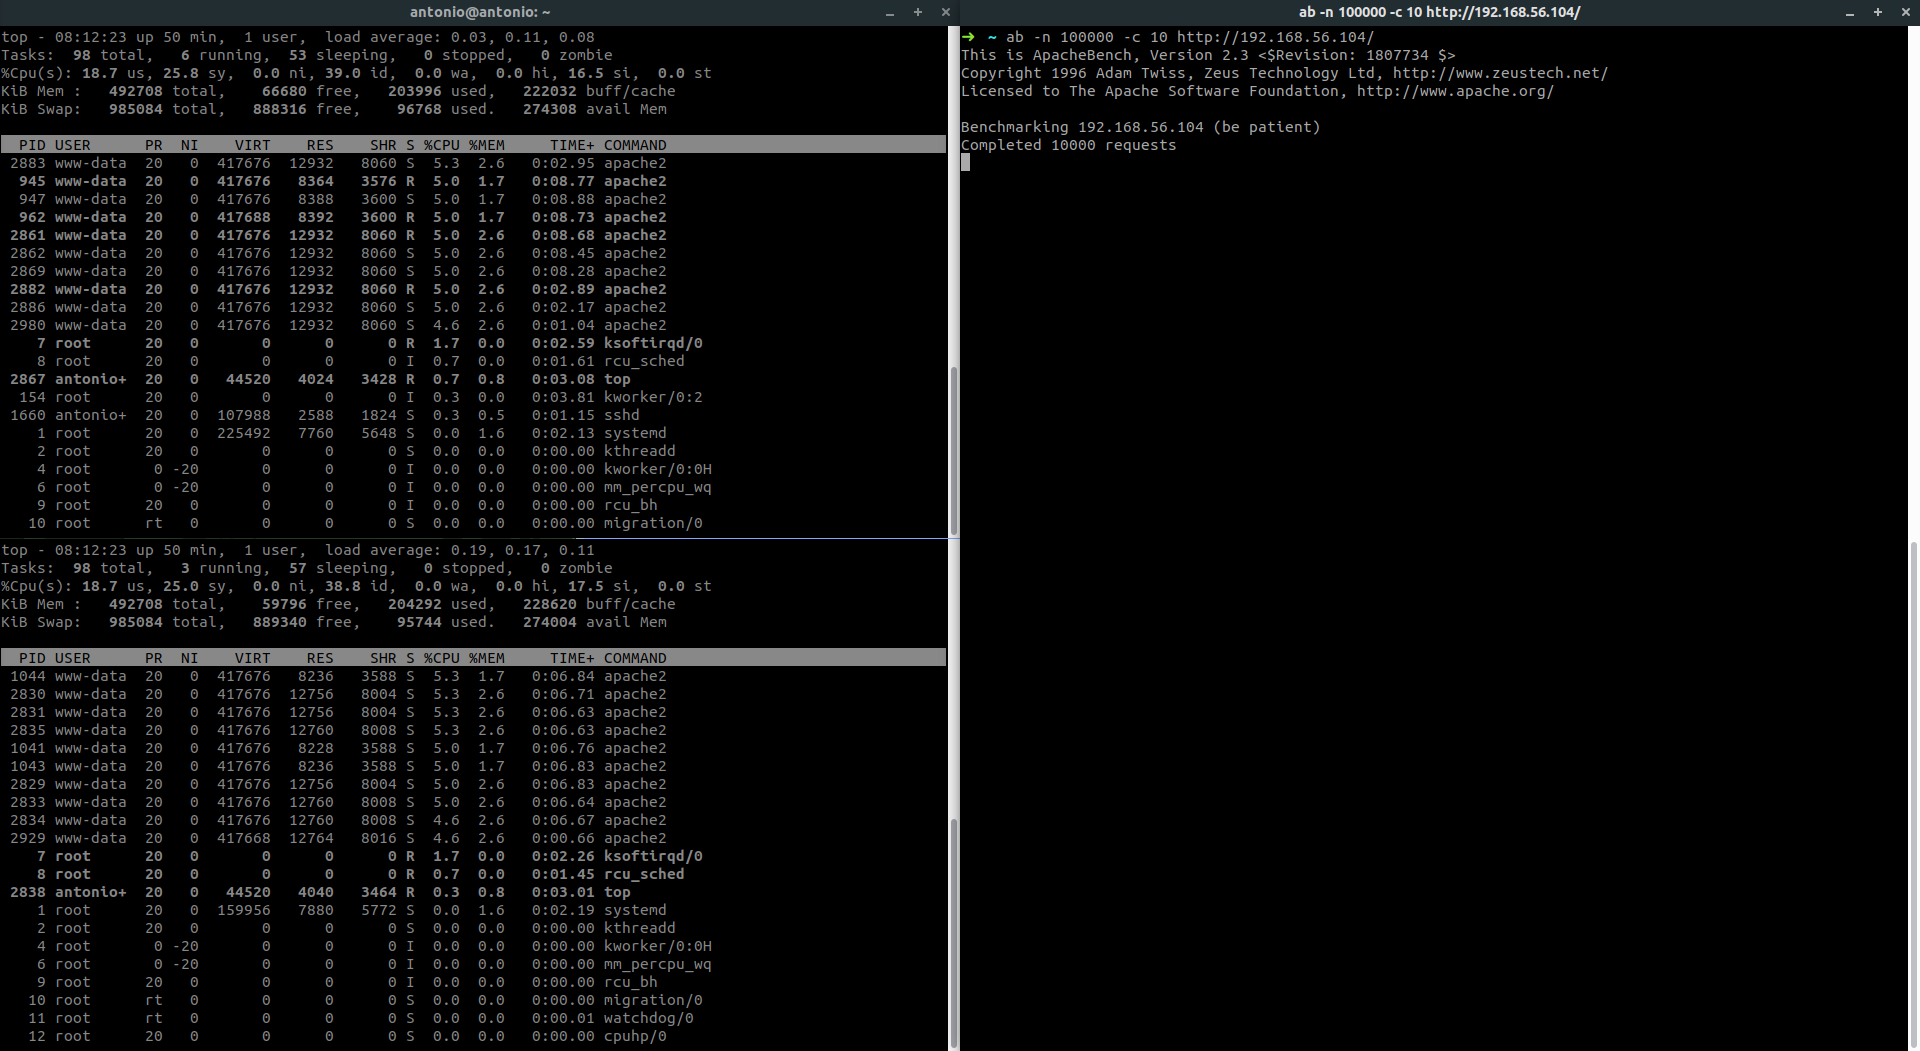
\includegraphics[scale=0.2]{20.png}
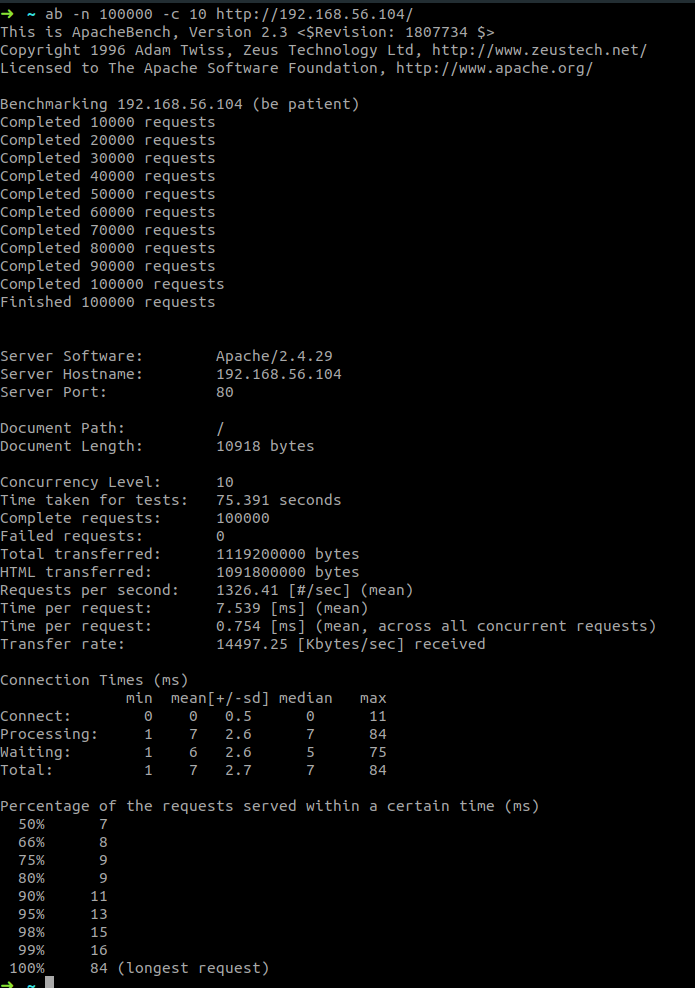
\includegraphics[scale=0.3]{21.png}
\end{figure}

Apagamos \textit{haproxy} y arrancamos \textit{nginx}:

\begin{figure}[H]
\center
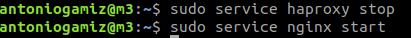
\includegraphics[scale=0.5]{19.png}
\end{figure}

\subsection{nginx}

\begin{figure}[H]
\center
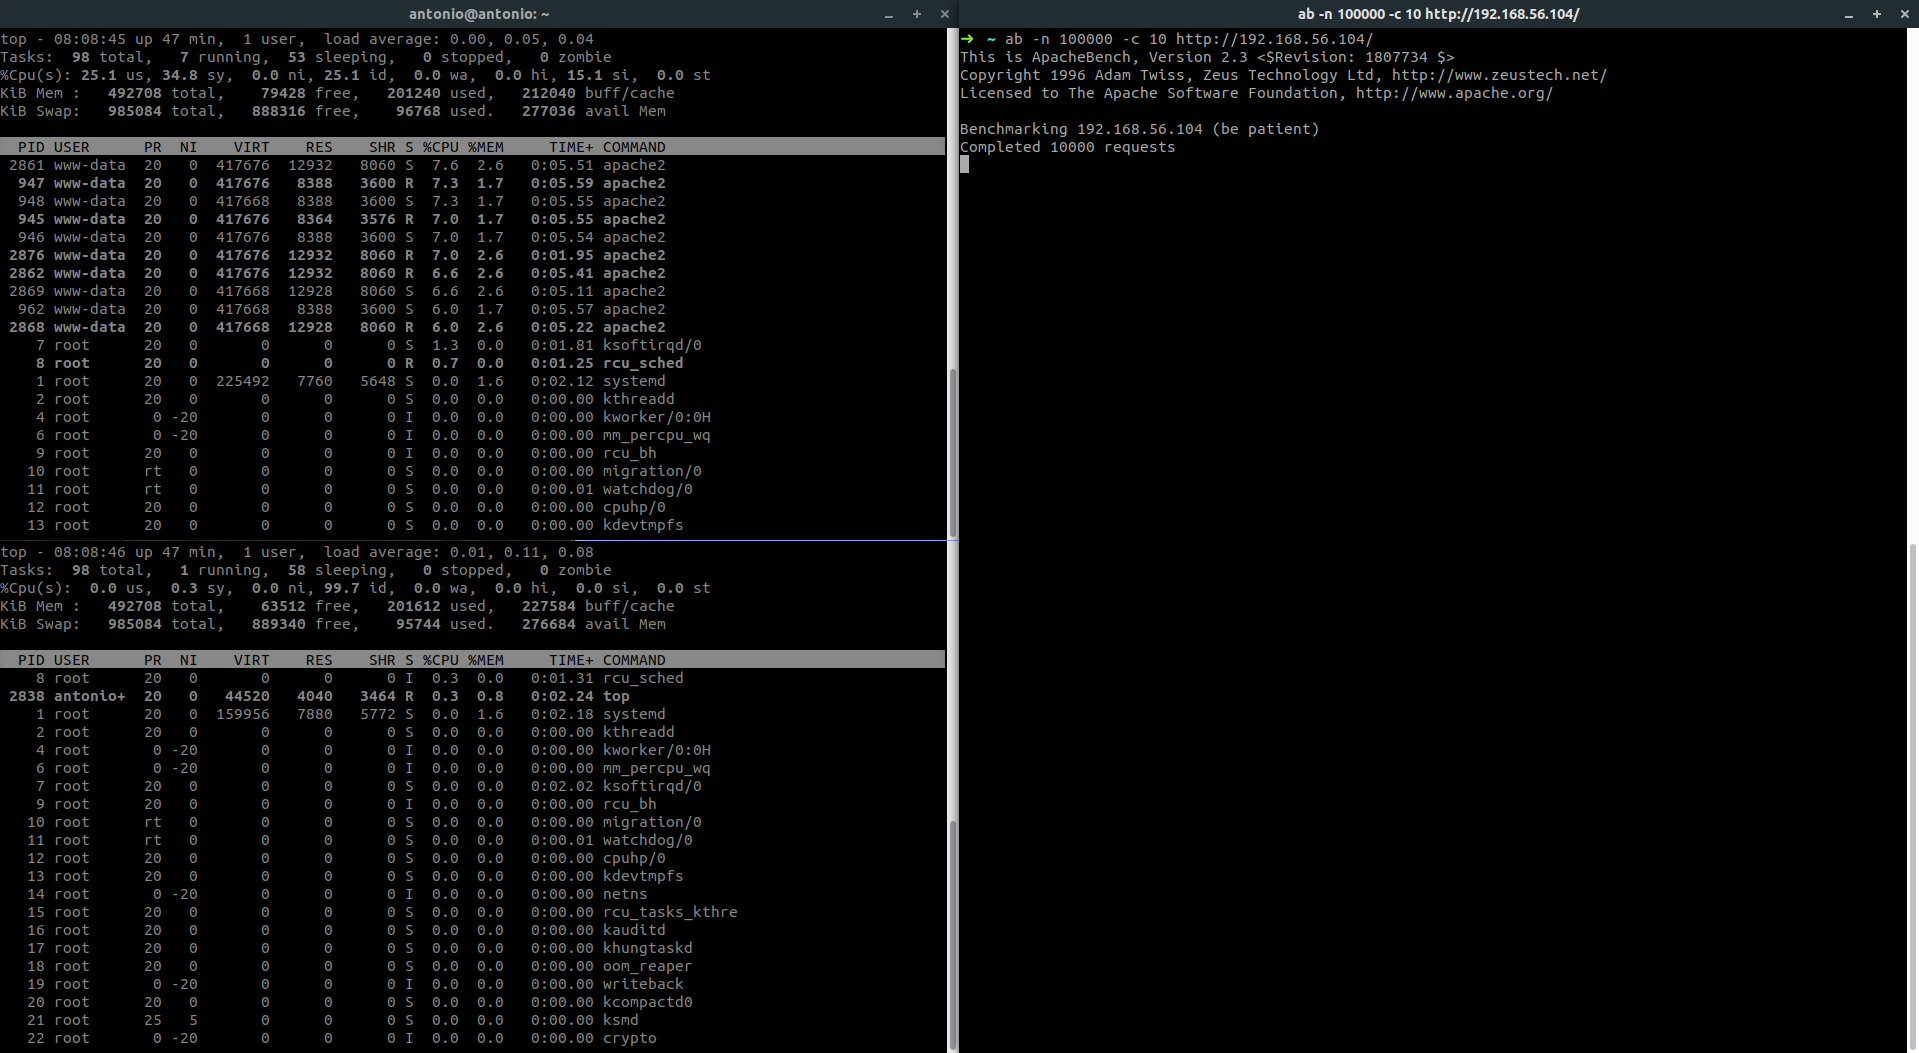
\includegraphics[scale=0.2]{17.png}
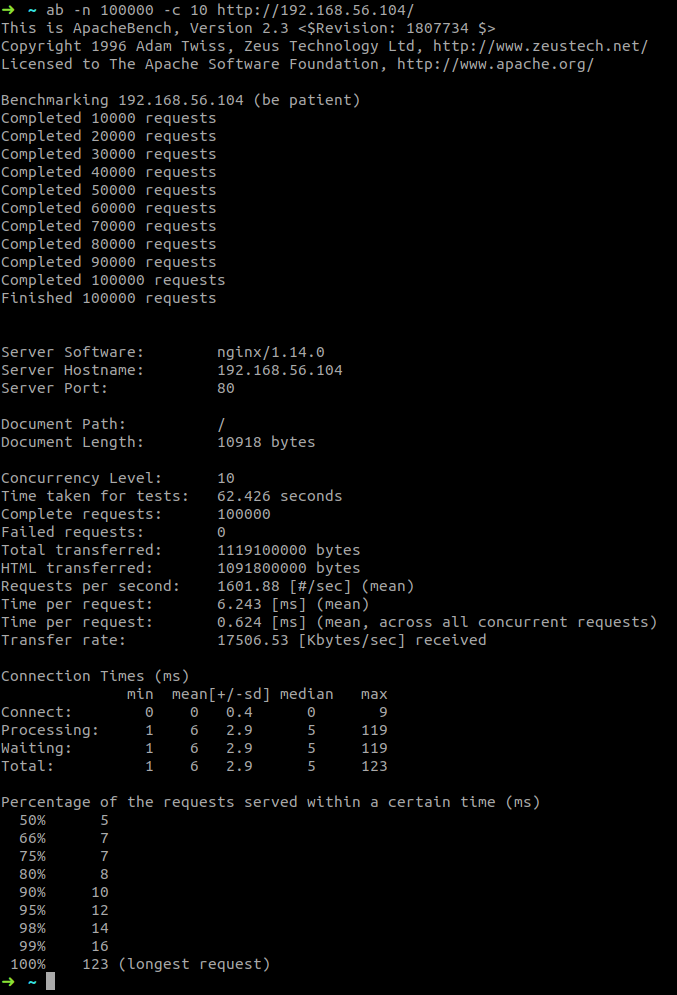
\includegraphics[scale=0.3]{18.png}
\end{figure}

\subsection{lighttpd}

\begin{figure}[H]
\center
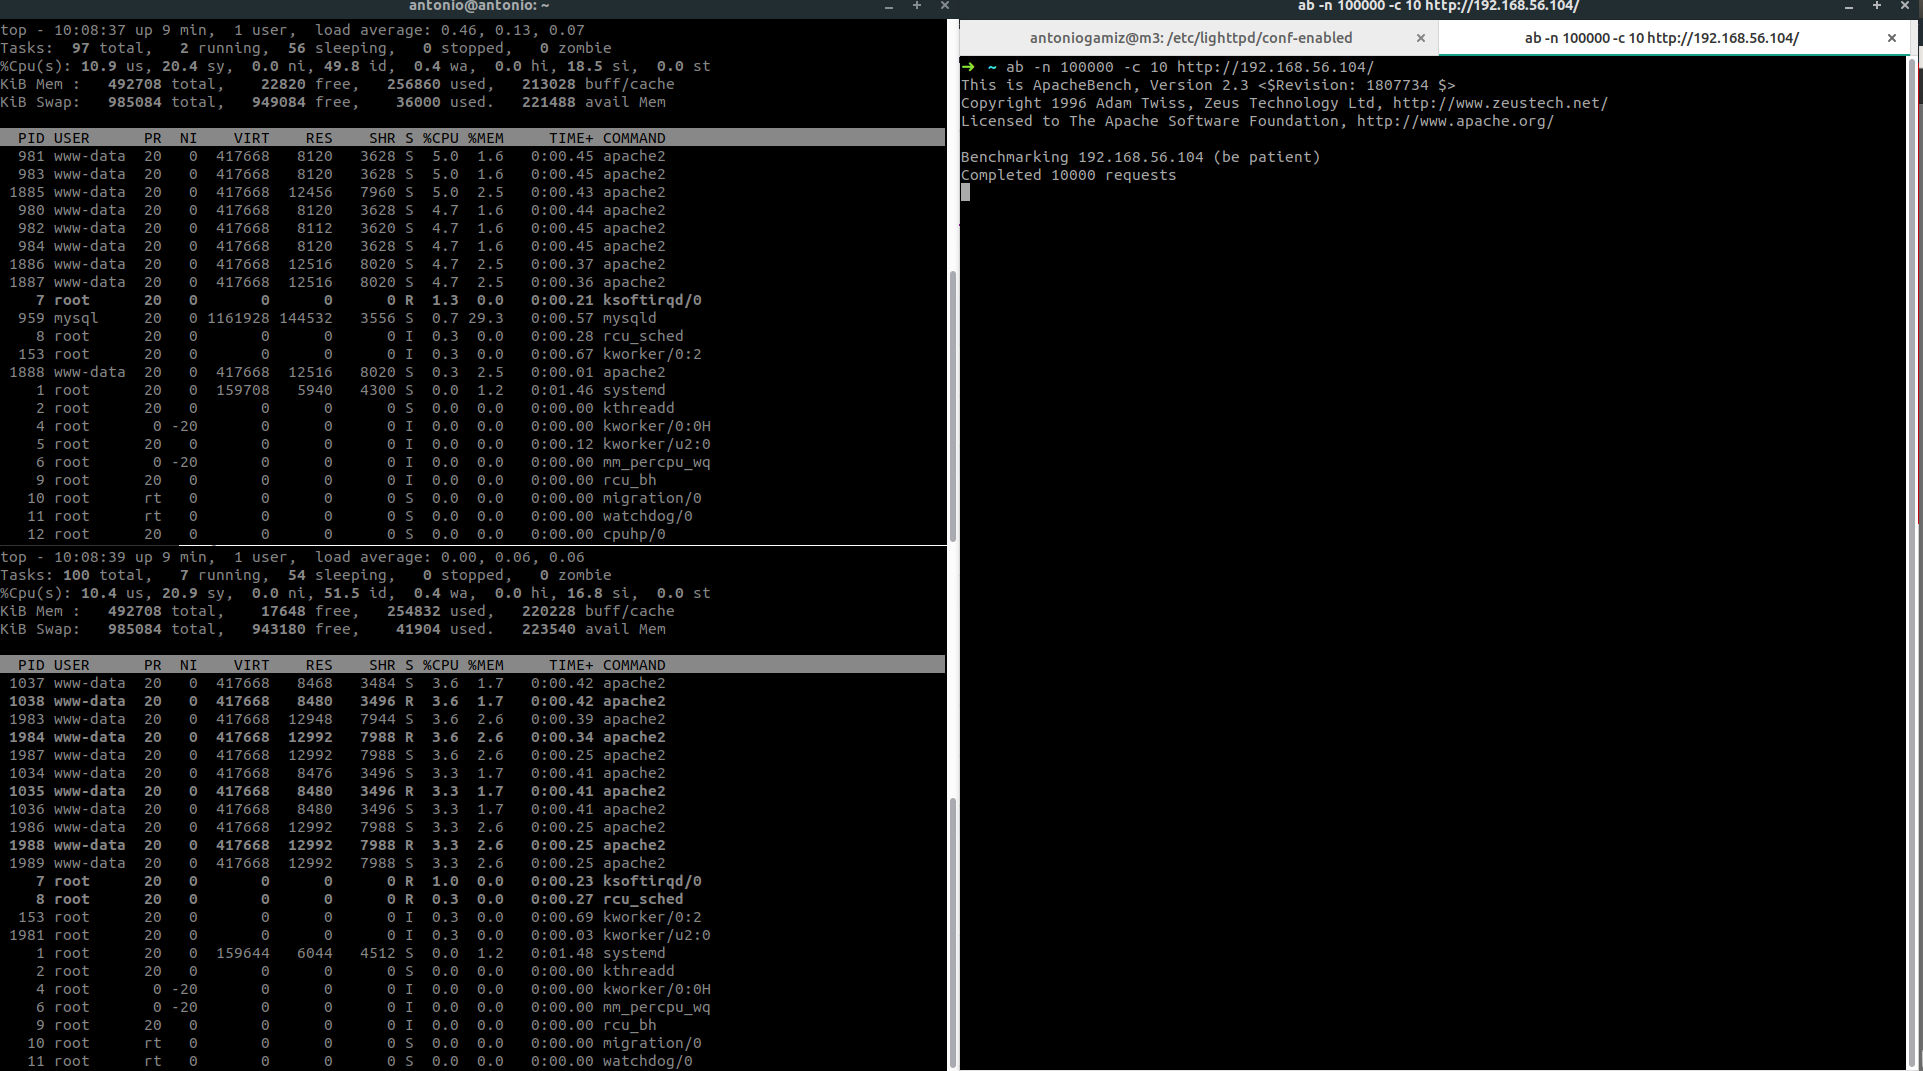
\includegraphics[scale=0.2]{30.png}
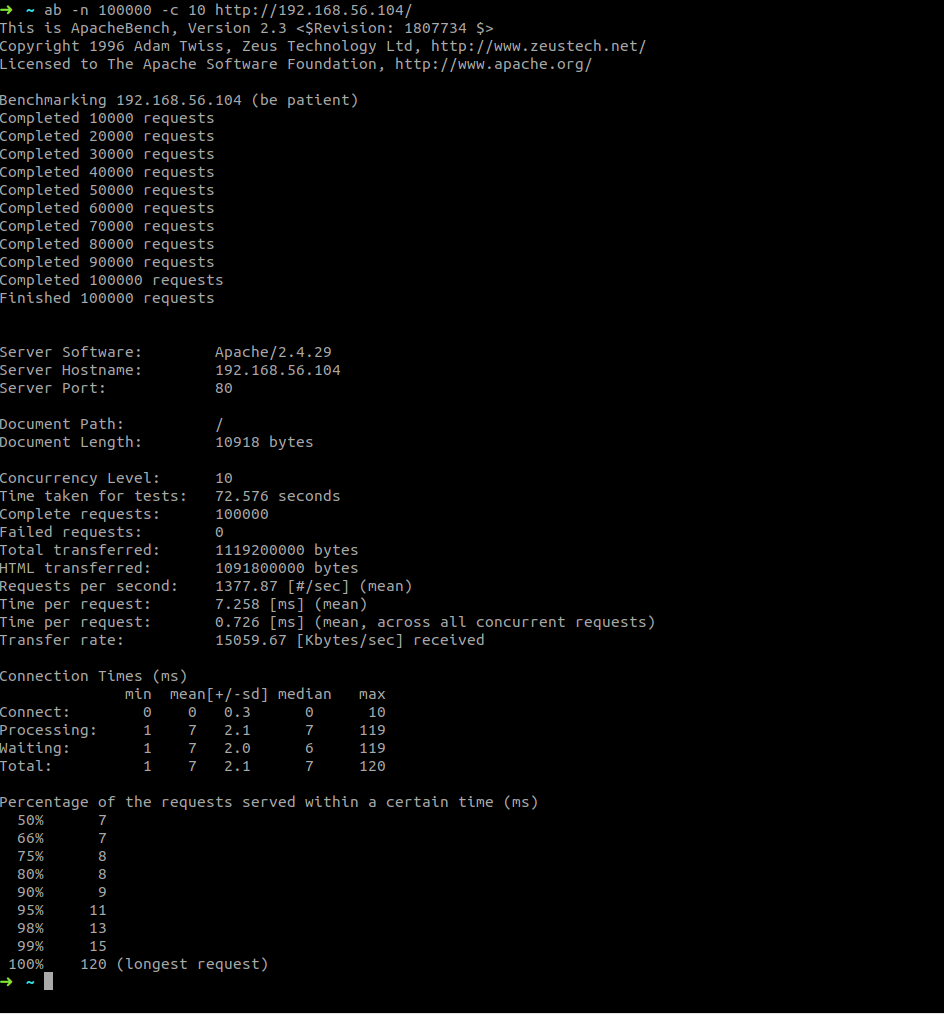
\includegraphics[scale=0.3]{31.png}
\end{figure}

\newpage

\section{Conclusión}

Después de haber instalado los 3 balanceadores y haberlos sometido a una carga de 100000 peticiones, podemos ver conjuntamente los resultados:

\begin{figure}[H]
\center
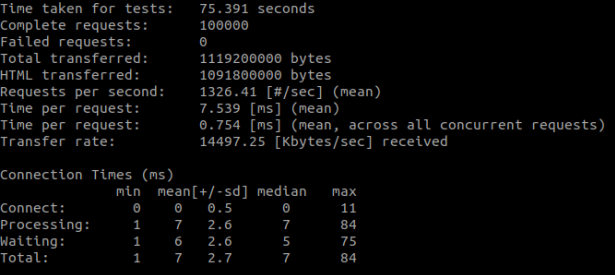
\includegraphics[scale=0.4]{32.png}
\caption{haproxy}
\medskip
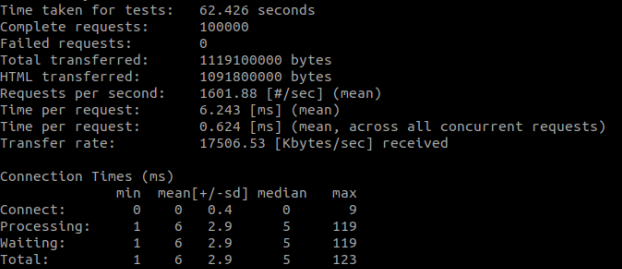
\includegraphics[scale=0.4]{33.png}
\caption{nginx}
\medskip
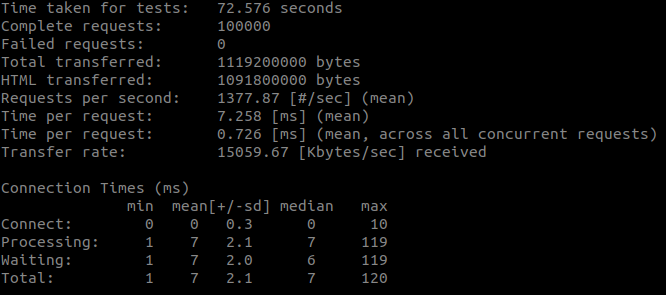
\includegraphics[scale=0.4]{34.png}
\caption{lighttpd}
\end{figure}

Como vemos, el que más rápido ha terminado ha sido \textit{nginx}, seguido por \textit{lighttpd} y por último \textit{haproxy}. La diferencia de tiempo entre \textit{nginx} y los dos anteriores es bastante significativa (unos 10 segundos), por lo que los datos muestran que, en esta prueba, \textit{nginx} es el más rápido.

\begin{thebibliography}{9}
\bibitem{lighttpd}
https://www.lighttpd.net/

\bibitem{lighttpd docs}
https://redmine.lighttpd.net/projects/lighttpd/wiki/Docs

\bibitem{StackOverflow}
https://stackoverflow.com/questions/14256746/lighttpd-load-balancing-configuration

\bibitem{StackOverflow}
https://stackoverflow.com/questions/61006844/lighttpd-is-not-redireccting-my-http-traffic

\end{thebibliography}

\end{document}